\documentclass[tikz,border=8pt]{standalone}
\usepackage[T1]{fontenc}
\usepackage[utf8]{inputenc}
\usepackage[sc]{mathpazo}
\usepackage{amsmath,amssymb}
\usepackage{xcolor}
\usepackage{tikz}
\usetikzlibrary{arrows.meta,calc,positioning,fit,backgrounds,decorations.pathmorphing}

\definecolor{cmjcrimson}{RGB}{155,20,30}
\definecolor{cmjgold}{RGB}{186,145,40}
\definecolor{cmjdark}{RGB}{35,35,35}
\definecolor{cmjgray}{RGB}{128,128,128}

\begin{document}
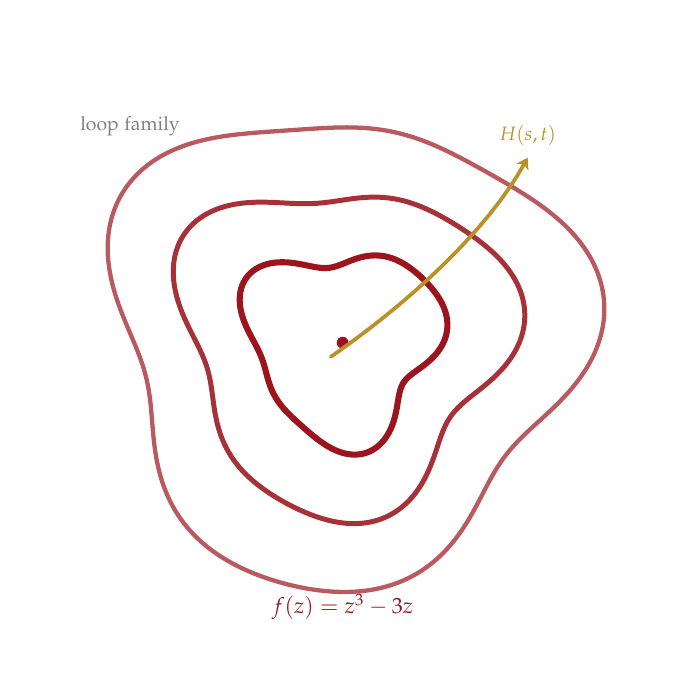
\begin{tikzpicture}[>=Stealth, line cap=round, line join=round, font=\small]
  \path[use as bounding box] (-4,-4) rectangle (4,4); % square canvas only
  % Title: Homotopy of Loops in Polynomial Geometry
  % Figure illustrates a continuous family of closed loops whose deformation reveals global structure.
  % no rendered title at the top
  % no visible frame box, no dashed guide frame, no center crosshair

  \draw[cmjcrimson, line width=2.2pt]
    plot[smooth cycle, samples=200, domain=0:360]
    ({(1.20 + 0.20*sin(3*\x) + 0.08*cos(5*\x))*cos(\x)},
     {(1.20 + 0.20*sin(3*\x) + 0.08*cos(5*\x))*sin(\x)});

  \draw[cmjcrimson, line width=1.8pt, opacity=0.88]
    plot[smooth cycle, samples=220, domain=0:360]
    ({(2.05 + 0.28*sin(3*\x + 18) + 0.11*cos(5*\x - 14))*cos(\x)},
     {(2.05 + 0.28*sin(3*\x + 18) + 0.11*cos(5*\x - 14))*sin(\x)});

  \draw[cmjcrimson, line width=1.55pt, opacity=0.70]
    plot[smooth cycle, samples=240, domain=0:360]
    ({(2.95 + 0.33*sin(3*\x + 34) + 0.13*cos(5*\x - 26))*cos(\x)},
     {(2.95 + 0.33*sin(3*\x + 34) + 0.13*cos(5*\x - 26))*sin(\x)});

  \fill[cmjcrimson] (0,0) circle (0.075);

  \draw[cmjgold, line width=1.35pt, -{Stealth[length=4pt,width=5pt]}]
    (-0.15,-0.18) .. controls (0.90,0.55) and (1.85,1.45) .. (2.35,2.35);

  \node[cmjgray, font=\scriptsize] at (-2.70,2.75) {loop family};
  \node[cmjgold, font=\scriptsize\bfseries] at (2.35,2.63) {$H(s,t)$};
  \node[cmjcrimson, font=\footnotesize] at (0,-3.35) {$f(z)=z^3-3z$};

\end{tikzpicture}
\end{document}
